\documentclass[11pt]{article}
\usepackage[a4paper,margin=1.8cm]{geometry}
\usepackage[T1]{fontenc}
\usepackage{lmodern}
\usepackage[protrusion=false,expansion=false]{microtype}
\DisableLigatures[-]{family=tt*}
\usepackage{booktabs}
\usepackage{array}
\usepackage{longtable}
\usepackage{graphicx}
\usepackage{amsmath}
\usepackage[hidelinks]{hyperref}
\usepackage{caption}
\captionsetup{font=small}
\usepackage[table]{xcolor}
\definecolor{muted}{HTML}{57606A}
\definecolor{todo}{HTML}{CF222E}
\definecolor{notebg}{HTML}{FFF8E5}
\definecolor{destmain}{HTML}{1F6FEB}
\definecolor{destsupp}{HTML}{2DA44E}
\definecolor{destnone}{HTML}{8C959F}
\emergencystretch=3em

% Destination tags, as in ../hg002-tiered-annotation.
\newcommand{\dest}[3]{%
  \par\medskip\noindent{\setlength{\fboxrule}{0.6pt}\fcolorbox{#1}{#1!8}{%
  \parbox{\dimexpr\textwidth-2\fboxsep-2\fboxrule}{%
  \textbf{\textcolor{#1}{#2}}\quad\small #3}}}\par\medskip}
\newcommand{\destmain}[1]{\dest{destmain}{$\rightarrow$ MAIN TEXT}{#1}}
\newcommand{\destsupp}[1]{\dest{destsupp}{$\rightarrow$ SUPPLEMENTARY}{#1}}
\newcommand{\destnone}[1]{\dest{destnone}{NOT FOR THE PAPER}{#1}}

\title{Ensembl VEP and its reimplementations:\\
a comparison table for Figure~1A\\[4pt]
\large Working document: panel, caption, Discussion fragment,
supplementary table, sources and notes}
\author{vepyr paper}
\date{17 October 2026}

\begin{document}
\maketitle

\noindent\colorbox{notebg}{\parbox{\dimexpr\textwidth-2\fboxsep}{\small
\textbf{How this was made.} The cells for fastVEP and vep-rs come from their
preprints and from their repositories at the commits listed in
Section~\ref{sec:sources}, read on 17~October~2026; field counts are taken
from their source code and documentation, not from running the tools. The
vepyr cells come from the main text and supplement of this paper. All
tables and the panel are generated from one data file
(\texttt{paper/tool-comparison/build\_table.py}); the panel is typeset in
Arial to match Figure~1 and exported as PDF, PNG and SVG. Speed is
deliberately left out: the published timings use different hardware, VEP
versions, VEP modes and annotation scopes, and are not comparable.}}

\tableofcontents

%% ===================================================================
\clearpage
\section{Figure 1A: compact comparison}
\label{sec:panel}
\destmain{Figure~1, first panel (\texttt{panel-tools.\{pdf,png,svg\}};
\texttt{panel-tools-nonotes.*} if the footnotes go to the caption). The
concordance row is a placeholder until the chromosome~22 comparison with
the merged cache has been run for all three reimplementations.}

\begin{center}
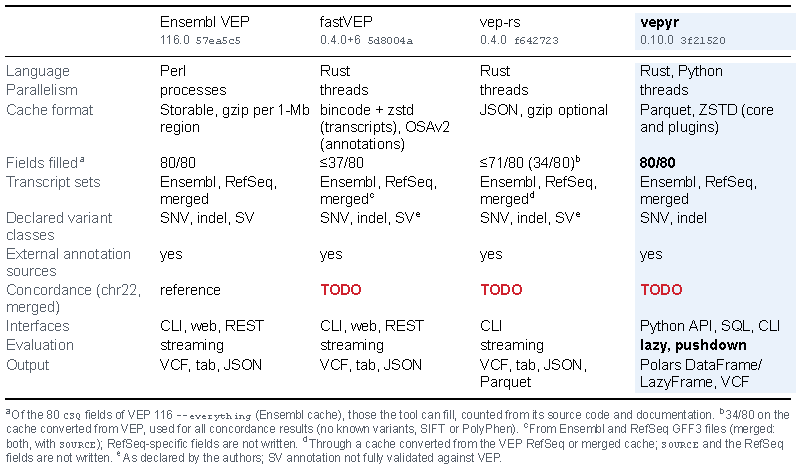
\includegraphics[width=\textwidth]{panel-tools.pdf}
\end{center}

\paragraph{Caption draft.} \textbf{(A)} Ensembl VEP and three
reimplementations. \emph{Fields filled}: of the 80 \texttt{CSQ} fields that
VEP~116 writes with \texttt{--everything} and the Ensembl cache, those that
each tool can fill. \emph{Declared variant classes}: as stated by the
authors of each tool. \emph{External annotation sources}: annotation from
data outside the core cache (VEP plugins and custom files in VEP, fastSA
sources in fastVEP, built-in plugins in vep-rs, plugin manifests in vepyr).
\emph{Concordance}: agreement with VEP on chromosome~22 of HG002 with the
merged cache, measured with the same inputs for all tools
[\textcolor{red}{TODO}]. \emph{Evaluation}: streaming tools process the
input in fixed batches; in vepyr, annotation is a lazy query whose columns
and genomic predicates determine the annotation work. Versions, sources and
the full comparison are given in Supplementary Table~Sx.

%% ===================================================================
\clearpage
\section{Main text: Discussion fragment}
\label{sec:discussion}
\destmain{Discussion or Conclusion, positioning vepyr against the other
reimplementations (about 150 words). Cite the two preprints.}

Two Rust reimplementations of VEP have been described recently, fastVEP and
vep-rs (Figure~1A). Both replace the VEP command line and report agreement
with VEP on consequence terms or on a subset of fields. fastVEP builds
transcript models from GFF3 and fills at most 37 of the 80
\texttt{--everything} fields; vep-rs reads its own JSON cache, which, when
converted from the VEP cache, carries no known variants or protein
predictions. vepyr takes a different route. It converts the complete
official cache, so that known variants, population frequencies, protein
predictions, regulatory features and RefSeq-specific fields are retained; its
output is byte-identical to that of VEP for a whole genome, including
plugins and transcript selection; and annotation is a lazy DataFrame
operation whose cost depends on the query. Its scope is narrower: human
GRCh38, small variants and six data-backed plugins. Structural variants,
supported by both other tools, are the main missing class; neither tool
reports field-level concordance with VEP for them.

%% ===================================================================
\clearpage
\section{Supplementary table: full comparison}
\label{sec:supp}
\destsupp{Supplementary Table~Sx: every attribute with the evidence behind
the compact cells of Figure~1A. Requested attributes first (parallelism to
output formats), then the additional ones.}

{\footnotesize
\setlength{\tabcolsep}{3pt}
\renewcommand{\arraystretch}{1.08}
\begin{longtable}{@{}>{\raggedright\arraybackslash}p{2.2cm}>{\raggedright\arraybackslash}p{3.55cm}>{\raggedright\arraybackslash}p{3.55cm}>{\raggedright\arraybackslash}p{3.55cm}>{\raggedright\arraybackslash}p{3.55cm}@{}}
\toprule
\textbf{Attribute} & \textbf{Ensembl VEP}\newline{\footnotesize\color{muted}116.0\enspace\texttt{57ea5c5}} & \textbf{fastVEP}\newline{\footnotesize\color{muted}0.4.0+6\enspace\texttt{5d8004a}} & \textbf{vep-rs}\newline{\footnotesize\color{muted}0.4.0\enspace\texttt{f642723}} & \textbf{vepyr}\newline{\footnotesize\color{muted}0.10.0\enspace\texttt{3f21520}} \\
\midrule
\endfirsthead
\toprule
\textbf{Attribute} & \textbf{Ensembl VEP}\newline{\footnotesize\color{muted}116.0\enspace\texttt{57ea5c5}} & \textbf{fastVEP}\newline{\footnotesize\color{muted}0.4.0+6\enspace\texttt{5d8004a}} & \textbf{vep-rs}\newline{\footnotesize\color{muted}0.4.0\enspace\texttt{f642723}} & \textbf{vepyr}\newline{\footnotesize\color{muted}0.10.0\enspace\texttt{3f21520}} \\
\midrule
\endhead
\bottomrule
\endfoot
\textit{Parallelism} & multi-process (\texttt{--fork}) & multi-threaded (rayon, all cores, no thread option); batches of 1,024 records; known-variant lookup and output sequential & multi-threaded (rayon; \texttt{--fork} sets threads, default one per CPU up to 32); bounded reader--annotator--writer pipeline & multi-threaded workers over index-defined position windows; output independent of the number of workers \\[3pt]
\textit{Implementation language} & Perl & Rust; web interface in JavaScript & Rust & Rust engine (DataFusion, Arrow); Python API (PyO3) \\[3pt]
\textit{Cache format and source} & official cache: Storable/Sereal \texttt{.gz} files per 1-Mb region; optional tabix-indexed known variants & transcripts: own binary cache (bincode + zstd; 388\,MB for GRCh38) built from GFF3; annotations (fastSA): OSAv2 (\texttt{.osa2}, zstd-compressed chunks; v1 \texttt{.osa} still read); VEP cache read only for known variants (\texttt{all\_vars.gz}) & own JSON cache, one file per chromosome and 1-Mb region (\texttt{.json}; \texttt{.json.gz} also read), converted from the VEP Storable cache by a Perl script or built from Ensembl GFF3, GTF and FASTA; plugin data in memory-mapped \texttt{.vpd} files & Apache Parquet (ZSTD), partitioned by chromosome and entity, with page indexes; converted from the official VEP cache; prebuilt caches on Hugging Face with pinned revisions and manifests \\[3pt]
\textit{Cache coverage (\texttt{CSQ} fields of \texttt{--everything})} & reference: 80, 85 and 86 fields (\texttt{ensembl}, \texttt{refseq} and \texttt{merged} caches, release 116) & 49 \texttt{CSQ} fields, 44 of the 80; at most 37/80 filled (motif fields have no writer, SIFT and PolyPhen always empty); no per-population frequencies, UniProt, \texttt{DOMAINS}, \texttt{VARIANT\_CLASS} & the 80 fields in the header; 9 always empty (motif, \texttt{DOMAINS}, \texttt{miRNA}, \texttt{UNIPARC}, \texttt{UNIPROT\_ISOFORM}): at most 71/80; converted cache has no known variants or SIFT/PolyPhen: 34/80 & all: 80/80, 85/85, 86/86 fields; 42 plugin fields \\[3pt]
\textit{Functional scope} & SNVs, indels, SVs and CNVs; regulatory and motif features; all \texttt{--everything} options & SNVs, indels, MNVs, SVs (DEL, DUP, INV, CNV, BND, INS, STR); mitochondria; ACMG classification; \texttt{--everything} accepted without effect; regulatory annotation not connected & SNVs, indels, MNVs, SVs (DEL, INS, DUP, INV, CNV, BND, mobile elements); mitochondria; no regulatory annotation; \texttt{--custom}, \texttt{--mirna}, \texttt{--hgvsg} accepted without effect & SNVs and short indels; regulatory and motif features; \texttt{--everything} always on; no SVs \\[3pt]
\textit{Concordance with VEP: published evidence and metric} & reference implementation & exact match of 22 of 24 fields on 2,920 transcript--allele pairs of the 173-variant VEP example (VEP 115.1, \texttt{--gff} mode); consequences and HGVS 99.49--100\% on ClinVar (6,600 variants) and HG002 (1 in 200) samples; pairs present in one tool only not scored; 9 deliberate divergences; SVs not compared & F1 over (location, allele, feature, consequence set) tuples, default options: $\ge$0.999974 on $2.6\times10^{8}$ tuples (VEP 115.2, preprint), 0.9999984 on $1.2\times10^{10}$ tuples (VEP 116.2, repository); all formats field for field on test corpora; SVs: F1 0.90--0.98 on chromosome~21 sets, no field comparison; not byte-identical & strict md5 of all record lines identical to VEP~116.0 on HG002 chr1--22 (4,096,123 records): 3 cache types, 5 plugins + ClinVar, 7 transcript-selection profiles (chr1, chr22); 205 tests ported from VEP \\[3pt]
\textit{Concordance on chr22, merged cache} & reference & \textcolor{todo}{\textbf{TODO}} & \textcolor{todo}{\textbf{TODO}} & \textcolor{todo}{\textbf{TODO}} \\[3pt]
\textit{User interfaces} & CLI; web interface; REST API & CLI; web interface and REST API (\texttt{fastvep-web}); release binaries (Linux x86-64, macOS arm64) & CLI with VEP option names (\texttt{--json\_cache} required); Docker image (amd64) & Python API (Polars) and SQL; CLI with VEP option names; nf-core module and subworkflow \\[3pt]
\textit{Lazy evaluation and streaming} & streaming in buffers (\texttt{--buffer\_size}, default 5,000); no lazy evaluation or pushdown & streaming in batches of 1,024 records; whole transcript set loaded (subset if the GFF3 is indexed); no region selection or pushdown & streaming in buffers through a bounded pipeline; transcripts loaded per chromosome, known variants loaded in full; no region selection or pushdown & lazy Polars source: projection pushdown (optional annotation work), region pushdown through the VCF index, row limit; streaming sinks \\[3pt]
\textit{Output formats} & VEP default (tab-delimited), VCF (\texttt{CSQ}), tab, JSON; HTML statistics & VCF (\texttt{CSQ} and \texttt{FV\_*} fields), tab (17 columns), JSON (VEP and Nirvana style) & VEP default, tab, VCF, JSON; Parquet through an external DuckDB process & Polars \texttt{LazyFrame}/\texttt{DataFrame} with typed columns; VCF (\texttt{CSQ}; plain, gzip, BGZF); Parquet and other formats through Polars sinks \\[3pt]
\textit{Transcript sets} & Ensembl, RefSeq, merged; GFF/GTF & Ensembl, RefSeq or merged from GFF3 files (\texttt{--gff3} repeated, per-transcript \texttt{SOURCE}); RefSeq-specific fields (\texttt{REFSEQ\_MATCH}, \texttt{BAM\_EDIT}, \ldots) not written & Ensembl; RefSeq and merged through a cache converted from the corresponding VEP cache (\texttt{--refseq} and \texttt{--merged} have no effect), but \texttt{SOURCE} and the RefSeq fields (\texttt{REFSEQ\_MATCH}, \texttt{BAM\_EDIT}, \ldots) are not written and the RefSeq BAM-edit correction is not implemented (open items of the project's parity matrix); no RefSeq concordance reported & Ensembl, RefSeq, merged \\[3pt]
\textit{Transcript selection (\texttt{--pick} etc.)} & \texttt{--pick}, \texttt{--per\_gene}, \texttt{--flag\_pick}, \texttt{--most\_severe} and others & \texttt{--pick} family (since 0.4.0) & \texttt{--pick} family; \texttt{--pick\_order} accepted without effect & \texttt{pick}, \texttt{pick\_allele}, \texttt{per\_gene}, \texttt{pick\_allele\_gene}, 3 \texttt{flag\_pick} variants \\[3pt]
\textit{External annotation sources} & 83 Perl plugin modules (\texttt{VEP\_plugins}, release 116); \texttt{--custom} (VCF, BED, GFF/GTF, bigWig) & fastSA: 18 built-in sources (ClinVar, gnomAD, dbNSFP, SpliceAI, AlphaMissense, REVEL, \ldots) and custom VCF/BED; no VEP plugins & 11 built-in plugins (CADD, REVEL, AlphaMissense, SpliceAI, LoFTEE, \ldots); C-ABI shared-library plugins; no \texttt{--custom} & declarative TOML manifests (TSV, CSV, Parquet, VCF, BED; SQL ingestion): CADD, SpliceAI, AlphaMissense, dbNSFP, PhenotypeOrthologous, ClinVar; no executable plugins \\[3pt]
\textit{Filtering of results (\texttt{filter\_vep})} & \texttt{filter\_vep} (own filter language) & \texttt{fastvep filter} & none & Polars expressions or SQL; 18 \texttt{filter\_vep} queries reproduced exactly \\[3pt]
\textit{Distribution} & GitHub (\texttt{INSTALL.pl}), Docker, Singularity, Bioconda; nf-core module & GitHub releases; conda recipe not on Bioconda; no container image & GitHub releases; Docker (ghcr.io) & PyPI wheels (Linux, macOS, Windows), Bioconda, nf-core \\[3pt]
\textit{Species, assemblies, VEP releases} & all Ensembl species; GRCh37 and GRCh38 & any organism with GFF3 and FASTA (5 benchmarked); GRCh37, GRCh38 & \textit{Homo sapiens} GRCh37 and GRCh38; VEP 115.2 (preprint), 116.2 (repository) & \textit{Homo sapiens} GRCh38; VEP 115.2 and 116.0 \\[3pt]
\textit{Licence} & Apache-2.0 & Apache-2.0 & Apache-2.0 & Apache-2.0 \\[3pt]
\end{longtable}

}

\noindent{\small Versions and git commits (also in the column headers):
Ensembl VEP~116.0 (\texttt{ensembl-vep} tag \texttt{release/116.0},
\texttt{57ea5c5}; \texttt{VEP\_plugins} branch \texttt{release/116},
\texttt{59b34e5}); fastVEP default branch at \texttt{5d8004a} (11~October
2026, six commits after tag \texttt{v0.4.0}, \texttt{d728c46}) and preprint
version~2; vep-rs tag \texttt{v0.4.0} (\texttt{f642723}, 16~October 2026)
and preprint version~1; vepyr tag \texttt{0.10.0} (\texttt{3f21520}),
validated with \texttt{0.9.2} (\texttt{844464c}). Field counts refer to the 80 \texttt{CSQ}
fields of VEP~116 \texttt{--everything} with the Ensembl cache (85 with
RefSeq, 86 with the merged cache) and were obtained from the source code and
documentation of each tool.}

%% ===================================================================
\clearpage
\section{Sources}
\label{sec:sources}
\destsupp{References for the table and the Discussion; add to
\texttt{references.bib} after checking the final versions.}

\begin{itemize}
\item \textbf{Ensembl VEP.} McLaren W, et al. The Ensembl Variant Effect
  Predictor. \emph{Genome Biol} 17:122 (2016).
  \url{https://github.com/Ensembl/ensembl-vep} (tag \texttt{release/116.0},
  commit \texttt{57ea5c52340a});
  \url{https://github.com/Ensembl/VEP_plugins} (branch \texttt{release/116},
  commit \texttt{59b34e58b41c}, 83 plugin modules).
\item \textbf{fastVEP.} Huang K. fastVEP: a high-performance variant effect
  predictor implemented in Rust. \emph{bioRxiv}
  doi:10.64898/2026.04.14.718452, version~2 (9~August 2026; version~1, 16
  April 2026, was titled ``fastVEP: A Fast, Comprehensive Variant Effect
  Predictor Written in Rust''). \url{https://github.com/Huang-lab/fastVEP},
  commit \texttt{5d8004a72fb7} (11~October 2026; tag \texttt{v0.4.0} is
  \texttt{d728c46fbd67}). Licence Apache-2.0.
\item \textbf{vep-rs.} Porter M, Borkowski R. vep-rs: high-throughput Rust
  variant annotation with population-scale concordance to Ensembl VEP.
  \emph{bioRxiv} doi:10.64898/2026.09.22.753614, version~1 (28~September
  2026); formatted for \emph{Bioinformatics}.
  \url{https://github.com/natera-open-source/vep-rs}, tag \texttt{v0.4.0},
  commit \texttt{f64272326dee} (16~October 2026). Licence Apache-2.0.
\item \textbf{vepyr.} This paper: Methods; Supplementary sections Scope,
  Plugins, Pushdowns and Validation. \url{https://github.com/biodatageeks/vepyr},
  tag \texttt{0.10.0} (commit \texttt{3f2152004c86}); validation with tag
  \texttt{0.9.2} (commit \texttt{844464c6b580}).
\end{itemize}

\subsection*{Evidence for the compact cells}
{\small\sloppy
\begin{description}
\item[fastVEP, fields.] \texttt{DEFAULT\_CSQ\_FIELDS} has 49 names
  (\texttt{crates/fastvep-io/src/output.rs:472--522}), 44 of them among the
  80; the five motif fields have no writer (\texttt{output.rs:41--46}) and
  \texttt{sift}/\texttt{polyphen} are always \texttt{None}
  (\texttt{crates/fastvep-annotate/src/lib.rs:428--429}): at most 37/80.
  Missing: \texttt{VARIANT\_CLASS}, UniProt fields, \texttt{GENE\_PHENO},
  \texttt{DOMAINS}, \texttt{miRNA}, all 28 population frequency fields and
  \texttt{MAX\_AF(\_POPS)}. \texttt{--everything}, \texttt{--symbol},
  \texttt{--canonical} and \texttt{--buffer-size} are parsed and discarded
  (\texttt{crates/fastvep-cli/src/main.rs:343--353}).
\item[fastVEP, concordance.] README (``22 of the 24 compared CSQ fields
  agree on 100\% of 2,920 shared (allele, transcript) pairs from the
  173-variant VEP example set''; VEP v115.1 ``\texttt{--gff} mode''); ClinVar
  sample of 6,600 variants and 1-in-200 HG002 sample: consequence set
  99.96\%/100\%, HGVSc 99.97\%/99.98\%, HGVSp 99.49\%/99.99\%; rows present
  in one tool only are not scored. No SV is compared with VEP: the
  validation datasets exclude SVs, which are covered by unit tests only.
\item[vep-rs, fields.] The \texttt{--everything} header lists the 80 fields;
  regulatory and motif annotation is not implemented, \texttt{DOMAINS} is
  never populated, \texttt{miRNA}, \texttt{UNIPARC},
  \texttt{UNIPROT\_ISOFORM} and \texttt{HGVSg} are always empty
  (\texttt{docs/cli-reference.md}, ``Compatibility with Perl VEP''): at most
  71/80. ``A converted cache carries no variation data and no SIFT or PolyPhen
  matrices'' (\texttt{docs/cache-setup.md}), which empties a further 37
  fields: 34/80.
\item[vep-rs, transcript sets.] \texttt{--refseq} and \texttt{--merged}
  ``selects no transcript set (the transcript set is the
  \texttt{--json\_cache} contents)'' (\texttt{docs/cli-reference.md}); README:
  ``accepted but not implemented''. The Perl converter accepts any Storable
  cache directory, so RefSeq or merged transcripts can be loaded, but the
  field table has no \texttt{REFSEQ\_MATCH}, \texttt{REFSEQ\_OFFSET},
  \texttt{GIVEN\_REF}, \texttt{USED\_REF} or \texttt{BAM\_EDIT}, and
  \texttt{SOURCE} has no writer (it falls through to the plugin lookup and
  is empty; \texttt{crates/vep-io/src/output/fields.rs}). In the project's
  parity matrix (\texttt{tests/parity/matrix.tsv}) the rows \texttt{refseq},
  \texttt{merged}, \texttt{refseq-merged-cache-selection},
  \texttt{refseq-match-bam-edit-source-columns} and
  \texttt{bam-refseq-model-correction} are all \texttt{open}. All published
  concordance uses the converted Ensembl cache.
\item[vep-rs, concordance.] Preprint: F1 over (location, allele, feature,
  consequence set) tuples, $\ge$0.999974 on $2.6\times10^8$ tuples from six
  datasets, VEP~115.2 with default options; ``It does not certify VEP's other
  output fields, and no VEP plugin enters any measurement''. Repository: F1
  0.9999984 on $1.2\times10^{10}$ tuples (VEP~116.2). Outputs compared field
  for field on golden corpora with default flags; JSON ``not
  byte-identical''. SVs: raw F1 0.975 (GRCh37) and 0.910 (GRCh38) on 16
  files per assembly (chromosome~21 and synthetic), ``no per-column
  comparator''.
\end{description}
}

%% ===================================================================
\clearpage
\section{Notes for the authors}
\label{sec:notes}
\destnone{Observations from reading the two preprints and repositories.}

\begin{enumerate}
\item \textbf{Make the field counts empirical.} The counts ($\le$37/80,
  $\le$71/80, 34/80) are read from source code and documentation. Before
  submission, run both tools on HG002 chromosome~22 with their closest
  equivalent of \texttt{--everything} and count the non-empty values per
  \texttt{CSQ} field; the table then rests on measured output, which is
  harder to dispute.
\item \textbf{Speed claims of the others are moving targets.} fastVEP
  version~2 withdrew the ``up to 130$\times$'' and ``$\sim$191$\times$''
  figures of version~1; it now reports 23.4$\times$ single-threaded on HG002
  against VEP~115.1 run in \texttt{--gff} mode (not with the cache), with
  the VEP genome time summed over per-chromosome runs. vep-rs reports
  78--284$\times$ against VEP~115.2 with \texttt{--fork 16} on AWS
  instances, and 5--14$\times$ against fastVEP. This supports leaving speed
  out of the comparison table and benchmarking on matched scope instead.
\item \textbf{vep-rs measured fastVEP.} On the same inputs, the vep-rs
  preprint reports fastVEP F1 of 0.762--0.970 on the six SNV/indel datasets
  and 0.13--0.15 on SVs, largely because its loader drops transcripts that
  the VEP cache holds. This is a third-party measurement; cite it only with
  attribution, if at all.
\item \textbf{Reproducing VEP's defects.} vep-rs documents behaviour of
  VEP~115 that it calls defects and does not reproduce (co-emission of
  \texttt{start\_lost} and \texttt{start\_retained\_variant},
  batch-dependent transcript selection for very large SVs, SV annotation
  against transcripts on another chromosome). Byte identity means vepyr
  reproduces whatever VEP writes for small variants, including the first of
  these. A reviewer may raise it; the position to state is that the goal is
  interchangeability with existing VEP outputs, filters and validated
  pipelines, and that any correction would have to be an explicit option.
\item \textbf{Scale and diversity of the concordance test.} vep-rs compares
  $1.2\times10^{10}$ tuples across ClinVar, gnomAD and 1000 Genomes, but on
  consequence terms only; vepyr compares all fields byte for byte, but on
  one genome (4.1 million records, three caches, plugins, transcript
  selection). A reviewer may ask for more variant diversity. A genome-wide
  ClinVar GRCh38 run (rich in indels and pathogenic coding variants) with the
  same strict md5 comparison would close that gap, before submission or in
  revision.
\item \textbf{Structural variants.} fastVEP supports SVs without any
  comparison with VEP; vep-rs compares SV consequence terms (not fields) on
  chromosome~21 and synthetic files. The table states vepyr's lack of SV
  support explicitly; if SV support is added in revision, it should be
  validated by the same standard before it enters the table.
\item \textbf{Moving repositories.} Both repositories changed substantially
  after their preprints (fastVEP: \texttt{--pick}, field counts; vep-rs: VEP
  116.2, whole-genome concordance). The table describes the repository state
  on 17~October 2026; update the cells and versions before submission
  (\texttt{build\_table.py}).
\item \textbf{vep-rs and VEP releases.} vep-rs~0.4.0 targets VEP~116.2;
  vepyr is validated against 116.0 (whole genome) and 116.2 (ported tests).
  The release-116 caches are the same, but the version difference should be
  stated if the two are compared directly.
\end{enumerate}

\end{document}
